\documentclass[11pt,a4paper]{article}
\usepackage[english]{babel}
% shared definitions (EN and HU); values come from generated/values_<lang>.tex
\usepackage[T1]{fontenc}
\usepackage[utf8]{inputenc}
\usepackage{lmodern}
\usepackage{textcomp}
\usepackage[margin=2.3cm]{geometry}
\usepackage{amsmath,amssymb}
\usepackage{booktabs}
\usepackage{graphicx}
\usepackage{microtype}
\usepackage[hidelinks]{hyperref}
\usepackage{fancyhdr}
\usepackage{lastpage}
\setlength{\footskip}{28pt}
\emergencystretch=3em
\makeatletter
\newcommand{\V}[1]{\ifcsname val@#1\endcsname\csname val@#1\endcsname\else\errmessage{missing value #1}\fi}
\let\tabinput\@@input
\makeatother
\newcommand{\um}{\ensuremath{\,\mu\mathrm{m}}}
\newcommand{\mmu}{\ensuremath{\,\mathrm{mm}}}
\newcommand{\cmu}{\ensuremath{\,\mathrm{cm}}}
\newcommand{\kmu}{\ensuremath{\,\mathrm{km}}}
\newcommand{\mU}{\ensuremath{\,\mathrm{m}}}
\newcommand{\kgu}{\ensuremath{\,\mathrm{kg}}}
\newcommand{\mss}{\ensuremath{\,\mathrm{m\,s^{-2}}}}
\newcommand{\uGal}{\ensuremath{\,\mu\mathrm{Gal}}}
\newcommand{\kgm}{\ensuremath{\,\mathrm{kg\,m^{-3}}}}
\newcommand{\Gu}{\ensuremath{\,\mathrm{m^{3}\,kg^{-1}\,s^{-2}}}}
\newcommand{\pct}{\,\%}
\newcommand{\degu}{\ensuremath{^\circ}}
\newcommand{\doi}[1]{\href{https://doi.org/#1}{\mbox{\nolinkurl{#1}}}}
\newcommand{\file}[1]{\nolinkurl{#1}}

\fancypagestyle{plain}{\fancyhf{}\renewcommand{\headrulewidth}{0pt}\fancyfoot[C]{\scriptsize\urlstyle{same}\begin{tabular}{@{}c@{}}\textcopyright\ 2026 Szabolcsi D\'avid (ORCID 0009-0005-6300-074X) \textperiodcentered\ CC BY-NC 4.0 International\\ \url{https://creativecommons.org/licenses/by-nc/4.0/}\\ commercial use only with the author's written permission \textperiodcentered\ page \thepage\ of \pageref{LastPage}\end{tabular}}}
\pagestyle{plain}
% generated by src/make_values.py from the module archives; do not edit
\expandafter\def\csname val@qAlpha\endcsname{\ensuremath{0.0795775}}
\expandafter\def\csname val@qCheck\endcsname{\ensuremath{0.0795775}}
\expandafter\def\csname val@LP1\endcsname{\ensuremath{10}}
\expandafter\def\csname val@aYP1\endcsname{\ensuremath{1}}
\expandafter\def\csname val@alphaP1\endcsname{\ensuremath{0.07958}}
\expandafter\def\csname val@aprimeP1\endcsname{\ensuremath{0.07371}}
\expandafter\def\csname val@GinfP1\endcsname{\ensuremath{0.926288}}
\expandafter\def\csname val@LP2\endcsname{\ensuremath{10}}
\expandafter\def\csname val@aYP2\endcsname{\ensuremath{1/3}}
\expandafter\def\csname val@alphaP2\endcsname{\ensuremath{0.02653}}
\expandafter\def\csname val@aprimeP2\endcsname{\ensuremath{0.02584}}
\expandafter\def\csname val@GinfP2\endcsname{\ensuremath{0.974160}}
\expandafter\def\csname val@LP3\endcsname{\ensuremath{1}}
\expandafter\def\csname val@aYP3\endcsname{\ensuremath{1}}
\expandafter\def\csname val@alphaP3\endcsname{\ensuremath{0.07958}}
\expandafter\def\csname val@aprimeP3\endcsname{\ensuremath{0.07371}}
\expandafter\def\csname val@GinfP3\endcsname{\ensuremath{0.926288}}
\expandafter\def\csname val@scal\endcsname{\ensuremath{0.10}}
\expandafter\def\csname val@scalLo\endcsname{\ensuremath{0.05}}
\expandafter\def\csname val@scalHi\endcsname{\ensuremath{0.20}}
\expandafter\def\csname val@Glab\endcsname{\ensuremath{6.6743\times10^{-11}}}
\expandafter\def\csname val@rIn\endcsname{\ensuremath{0.09}}
\expandafter\def\csname val@rOut\endcsname{\ensuremath{0.22}}
\expandafter\def\csname val@hSrc\endcsname{\ensuremath{0.50}}
\expandafter\def\csname val@rhoSrc\endcsname{\ensuremath{2700}}
\expandafter\def\csname val@Msrc\endcsname{\ensuremath{170.9}}
\expandafter\def\csname val@AB\endcsname{\ensuremath{1.60}}
\expandafter\def\csname val@xSone\endcsname{\ensuremath{-0.32}}
\expandafter\def\csname val@xStwo\endcsname{\ensuremath{1.92}}
\expandafter\def\csname val@dmin\endcsname{\ensuremath{0.10}}
\expandafter\def\csname val@DyGR\endcsname{\ensuremath{-6.247\times10^{-25}}}
\expandafter\def\csname val@DaGR\endcsname{\ensuremath{-9.793\times10^{-8}}}
\expandafter\def\csname val@nPanel\endcsname{\ensuremath{12}}
\expandafter\def\csname val@quadLo\endcsname{\ensuremath{-2}}
\expandafter\def\csname val@quadHi\endcsname{\ensuremath{5}}
\expandafter\def\csname val@boundLo\endcsname{\ensuremath{-5}}
\expandafter\def\csname val@perDec\endcsname{\ensuremath{8}}
\expandafter\def\csname val@perDecB\endcsname{\ensuremath{8}}
\expandafter\def\csname val@dyP1\endcsname{\ensuremath{1.432\times10^{-34}}}
\expandafter\def\csname val@daP1\endcsname{\ensuremath{7.355\times10^{-18}}}
\expandafter\def\csname val@dyRawP1\endcsname{\ensuremath{-4.97\times10^{-26}}}
\expandafter\def\csname val@daRawP1\endcsname{\ensuremath{-7.79\times10^{-9}}}
\expandafter\def\csname val@dyRelP1\endcsname{\ensuremath{-2.29\times10^{-10}}}
\expandafter\def\csname val@daRelP1\endcsname{\ensuremath{-7.51\times10^{-11}}}
\expandafter\def\csname val@dyLoP1\endcsname{\ensuremath{1.449\times10^{-34}}}
\expandafter\def\csname val@daLoP1\endcsname{\ensuremath{7.626\times10^{-18}}}
\expandafter\def\csname val@dyHiP1\endcsname{\ensuremath{1.363\times10^{-34}}}
\expandafter\def\csname val@daHiP1\endcsname{\ensuremath{6.273\times10^{-18}}}
\expandafter\def\csname val@aLimLabP1\endcsname{\ensuremath{4.53\times10^{-4}}}
\expandafter\def\csname val@RLabP1\endcsname{\ensuremath{175.6}}
\expandafter\def\csname val@aLimBrenAP1\endcsname{\ensuremath{8.31\times10^{-3}}}
\expandafter\def\csname val@aLimBrenBP1\endcsname{\ensuremath{7.92\times10^{-3}}}
\expandafter\def\csname val@aLimBrenCP1\endcsname{\ensuremath{8.29\times10^{-3}}}
\expandafter\def\csname val@RBrenMinP1\endcsname{\ensuremath{9.58}}
\expandafter\def\csname val@RBrenMaxP1\endcsname{\ensuremath{10.05}}
\expandafter\def\csname val@RConsP1\endcsname{\ensuremath{9.58}}
\expandafter\def\csname val@SyOcxoP1\endcsname{\ensuremath{1.4\times10^{-23}}}
\expandafter\def\csname val@SySrP1\endcsname{\ensuremath{1.9\times10^{-14}}}
\expandafter\def\csname val@SaGP1\endcsname{\ensuremath{4.1\times10^{-9}}}
\expandafter\def\csname val@SaPP1\endcsname{\ensuremath{7.5\times10^{-7}}}
\expandafter\def\csname val@maxSP1\endcsname{\ensuremath{7.51\times10^{-7}}}
\expandafter\def\csname val@catP1\endcsname{b}
\expandafter\def\csname val@dyKoneP1\endcsname{\ensuremath{-4.605\times10^{-26}}}
\expandafter\def\csname val@kcNeedP1\endcsname{\ensuremath{8.252\times10^{5}}}
\expandafter\def\csname val@dyP2\endcsname{\ensuremath{5.020\times10^{-35}}}
\expandafter\def\csname val@daP2\endcsname{\ensuremath{2.579\times10^{-18}}}
\expandafter\def\csname val@dyRelP2\endcsname{\ensuremath{-8.04\times10^{-11}}}
\expandafter\def\csname val@daRelP2\endcsname{\ensuremath{-2.63\times10^{-11}}}
\expandafter\def\csname val@dyLoP2\endcsname{\ensuremath{5.081\times10^{-35}}}
\expandafter\def\csname val@daLoP2\endcsname{\ensuremath{2.673\times10^{-18}}}
\expandafter\def\csname val@dyHiP2\endcsname{\ensuremath{4.778\times10^{-35}}}
\expandafter\def\csname val@daHiP2\endcsname{\ensuremath{2.199\times10^{-18}}}
\expandafter\def\csname val@aLimLabP2\endcsname{\ensuremath{4.53\times10^{-4}}}
\expandafter\def\csname val@RLabP2\endcsname{\ensuremath{58.55}}
\expandafter\def\csname val@aLimBrenAP2\endcsname{\ensuremath{8.31\times10^{-3}}}
\expandafter\def\csname val@aLimBrenBP2\endcsname{\ensuremath{7.92\times10^{-3}}}
\expandafter\def\csname val@aLimBrenCP2\endcsname{\ensuremath{8.29\times10^{-3}}}
\expandafter\def\csname val@RBrenMinP2\endcsname{\ensuremath{3.19}}
\expandafter\def\csname val@RBrenMaxP2\endcsname{\ensuremath{3.35}}
\expandafter\def\csname val@RConsP2\endcsname{\ensuremath{3.19}}
\expandafter\def\csname val@SyOcxoP2\endcsname{\ensuremath{5.0\times10^{-24}}}
\expandafter\def\csname val@SySrP2\endcsname{\ensuremath{6.6\times10^{-15}}}
\expandafter\def\csname val@SaGP2\endcsname{\ensuremath{1.4\times10^{-9}}}
\expandafter\def\csname val@SaPP2\endcsname{\ensuremath{2.6\times10^{-7}}}
\expandafter\def\csname val@maxSP2\endcsname{\ensuremath{2.63\times10^{-7}}}
\expandafter\def\csname val@catP2\endcsname{b}
\expandafter\def\csname val@dyKoneP2\endcsname{\ensuremath{-1.614\times10^{-26}}}
\expandafter\def\csname val@kcNeedP2\endcsname{\ensuremath{2.354\times10^{6}}}
\expandafter\def\csname val@dyP3\endcsname{\ensuremath{1.431\times10^{-32}}}
\expandafter\def\csname val@daP3\endcsname{\ensuremath{7.350\times10^{-16}}}
\expandafter\def\csname val@dyRelP3\endcsname{\ensuremath{-2.29\times10^{-8}}}
\expandafter\def\csname val@daRelP3\endcsname{\ensuremath{-7.51\times10^{-9}}}
\expandafter\def\csname val@dyLoP3\endcsname{\ensuremath{1.448\times10^{-32}}}
\expandafter\def\csname val@daLoP3\endcsname{\ensuremath{7.620\times10^{-16}}}
\expandafter\def\csname val@dyHiP3\endcsname{\ensuremath{1.362\times10^{-32}}}
\expandafter\def\csname val@daHiP3\endcsname{\ensuremath{6.267\times10^{-16}}}
\expandafter\def\csname val@aLimLabP3\endcsname{\ensuremath{5.94\times10^{-4}}}
\expandafter\def\csname val@RLabP3\endcsname{\ensuremath{134.0}}
\expandafter\def\csname val@aLimBrenAP3\endcsname{\ensuremath{9.52\times10^{-3}}}
\expandafter\def\csname val@aLimBrenBP3\endcsname{\ensuremath{9.47\times10^{-3}}}
\expandafter\def\csname val@aLimBrenCP3\endcsname{\ensuremath{9.52\times10^{-3}}}
\expandafter\def\csname val@RBrenMinP3\endcsname{\ensuremath{8.36}}
\expandafter\def\csname val@RBrenMaxP3\endcsname{\ensuremath{8.40}}
\expandafter\def\csname val@RConsP3\endcsname{\ensuremath{8.36}}
\expandafter\def\csname val@SyOcxoP3\endcsname{\ensuremath{1.4\times10^{-21}}}
\expandafter\def\csname val@SySrP3\endcsname{\ensuremath{1.9\times10^{-12}}}
\expandafter\def\csname val@SaGP3\endcsname{\ensuremath{4.1\times10^{-7}}}
\expandafter\def\csname val@SaPP3\endcsname{\ensuremath{7.5\times10^{-5}}}
\expandafter\def\csname val@maxSP3\endcsname{\ensuremath{7.51\times10^{-5}}}
\expandafter\def\csname val@catP3\endcsname{b}
\expandafter\def\csname val@dyKoneP3\endcsname{\ensuremath{-4.605\times10^{-26}}}
\expandafter\def\csname val@kcNeedP3\endcsname{\ensuremath{8.252\times10^{5}}}
\expandafter\def\csname val@aLimKN\endcsname{\ensuremath{0.0032}}
\expandafter\def\csname val@RKN\endcsname{\ensuremath{24.9}}
\expandafter\def\csname val@aLimBNsp\endcsname{\ensuremath{1.13\times10^{-3}}}
\expandafter\def\csname val@RBNsp\endcsname{\ensuremath{70.7}}
\expandafter\def\csname val@sigOcxo\endcsname{\ensuremath{1\times10^{-11}}}
\expandafter\def\csname val@sigBeat\endcsname{\ensuremath{2.56\times10^{-11}}}
\expandafter\def\csname val@sigSrSys\endcsname{\ensuremath{8.1\times10^{-19}}}
\expandafter\def\csname val@sigSrDiff\endcsname{\ensuremath{7.6\times10^{-21}}}
\expandafter\def\csname val@sigTors\endcsname{\ensuremath{3.1\times10^{-15}}}
\expandafter\def\csname val@epsG\endcsname{\ensuremath{0.0185}}
\expandafter\def\csname val@epsP\endcsname{\ensuremath{1\times10^{-4}}}
\expandafter\def\csname val@Sthr\endcsname{\ensuremath{5}}
\expandafter\def\csname val@MinFactor\endcsname{\ensuremath{6.662\times10^{4}}}
\expandafter\def\csname val@catRem\endcsname{c}
\expandafter\def\csname val@catBand\endcsname{c}
\expandafter\def\csname val@lamEdge\endcsname{\ensuremath{75.88}}
\expandafter\def\csname val@logDyEdge\endcsname{\ensuremath{-593.6}}
\expandafter\def\csname val@logDaEdge\endcsname{\ensuremath{-576.0}}
\expandafter\def\csname val@logDyPlus\endcsname{\ensuremath{-451.3}}
\expandafter\def\csname val@logDaPlus\endcsname{\ensuremath{-433.6}}
\expandafter\def\csname val@Rfifty\endcsname{\ensuremath{0.190}}
\expandafter\def\csname val@ImpFifty\endcsname{\ensuremath{5.3}}
\expandafter\def\csname val@lamFifty\endcsname{\ensuremath{50}}
\expandafter\def\csname val@xiTi\endcsname{\ensuremath{2.022\times10^{-3}}}
\expandafter\def\csname val@xiPt\endcsname{\ensuremath{4.054\times10^{-3}}}
\expandafter\def\csname val@etaNF\endcsname{\ensuremath{6.882\times10^{-15}}}
\expandafter\def\csname val@kcMax\endcsname{\ensuremath{4.255\times10^{-11}}}
\expandafter\def\csname val@nTests\endcsname{\ensuremath{16}}
\expandafter\def\csname val@nCtrl\endcsname{\ensuremath{5}}
\expandafter\def\csname val@rtolClock\endcsname{\ensuremath{8}}
\expandafter\def\csname val@brAlpha\endcsname{\ensuremath{0.0795775}}
\expandafter\def\csname val@brLam\endcsname{\ensuremath{10}}
\expandafter\def\csname val@zNull\endcsname{\ensuremath{9.8}}
\expandafter\def\csname val@zKEN\endcsname{\ensuremath{454}}
\expandafter\def\csname val@zBN\endcsname{\ensuremath{457.15}}
\expandafter\def\csname val@hKN\endcsname{\ensuremath{465}}
\expandafter\def\csname val@Rtrunc\endcsname{\ensuremath{240}}
\expandafter\def\csname val@nRings\endcsname{\ensuremath{45}}
\expandafter\def\csname val@nStations\endcsname{\ensuremath{1838}}
\expandafter\def\csname val@nGrid\endcsname{\ensuremath{301}}
\expandafter\def\csname val@cellM\endcsname{\ensuremath{180}}
\expandafter\def\csname val@nPrisms\endcsname{\ensuremath{103728}}
\expandafter\def\csname val@aEarth\endcsname{\ensuremath{6371}}
\expandafter\def\csname val@towerLat\endcsname{\ensuremath{36.78059}}
\expandafter\def\csname val@towerLon\endcsname{\ensuremath{116.24359}}
\expandafter\def\csname val@rho1800\endcsname{\ensuremath{1800}}
\expandafter\def\csname val@rho2000\endcsname{\ensuremath{2000}}
\expandafter\def\csname val@rho2200\endcsname{\ensuremath{2200}}
\expandafter\def\csname val@rho2670\endcsname{\ensuremath{2670}}
\expandafter\def\csname val@kRes\endcsname{\ensuremath{93}}
\expandafter\def\csname val@kSig\endcsname{\ensuremath{95}}
\expandafter\def\csname val@kSigma\endcsname{\ensuremath{1.96}}
\expandafter\def\csname val@edgeBEN\endcsname{\ensuremath{-279.2}}
\expandafter\def\csname val@yBN\endcsname{\ensuremath{3.5}}
\expandafter\def\csname val@sBN\endcsname{\ensuremath{40.3}}
\expandafter\def\csname val@edgeBN\endcsname{\ensuremath{-75.5}}
\expandafter\def\csname val@nbias\endcsname{\ensuremath{137.6}}
\expandafter\def\csname val@nbiasRep\endcsname{\ensuremath{140}}
\expandafter\def\csname val@nbiasRepSig\endcsname{\ensuremath{20}}
\expandafter\def\csname val@nbiasKEN\endcsname{\ensuremath{111.9}}
\expandafter\def\csname val@nbiasKENrep\endcsname{\ensuremath{100}}
\expandafter\def\csname val@wsum\endcsname{\ensuremath{-0.00197}}
\expandafter\def\csname val@topFlat\endcsname{\ensuremath{-2972.3}}
\expandafter\def\csname val@topA\endcsname{\ensuremath{-2766.9}}
\expandafter\def\csname val@topB\endcsname{\ensuremath{-2900.6}}
\expandafter\def\csname val@topOpA\endcsname{\ensuremath{133.9}}
\expandafter\def\csname val@topTerr\endcsname{\ensuremath{71.5}}
\expandafter\def\csname val@topTerrPct\endcsname{\ensuremath{2.4}}
\expandafter\def\csname val@RflatBEN2000\endcsname{\ensuremath{10.297}}
\expandafter\def\csname val@RABEN2000\endcsname{\ensuremath{9.580}}
\expandafter\def\csname val@RBBEN2000\endcsname{\ensuremath{10.046}}
\expandafter\def\csname val@RCBEN2000\endcsname{\ensuremath{9.605}}
\expandafter\def\csname val@RDBEN2000\endcsname{\ensuremath{9.580}}
\expandafter\def\csname val@RflatBN2000\endcsname{\ensuremath{38.564}}
\expandafter\def\csname val@RABN2000\endcsname{\ensuremath{35.894}}
\expandafter\def\csname val@RBBN2000\endcsname{\ensuremath{37.633}}
\expandafter\def\csname val@RCBN2000\endcsname{\ensuremath{35.986}}
\expandafter\def\csname val@RDBN2000\endcsname{\ensuremath{35.896}}
\expandafter\def\csname val@RflatBEN2200\endcsname{\ensuremath{11.334}}
\expandafter\def\csname val@RABEN2200\endcsname{\ensuremath{10.546}}
\expandafter\def\csname val@RBBEN2200\endcsname{\ensuremath{11.059}}
\expandafter\def\csname val@RCBEN2200\endcsname{\ensuremath{10.573}}
\expandafter\def\csname val@RDBEN2200\endcsname{\ensuremath{10.546}}
\expandafter\def\csname val@RflatBN2200\endcsname{\ensuremath{42.429}}
\expandafter\def\csname val@RABN2200\endcsname{\ensuremath{39.491}}
\expandafter\def\csname val@RBBN2200\endcsname{\ensuremath{41.404}}
\expandafter\def\csname val@RCBN2200\endcsname{\ensuremath{39.593}}
\expandafter\def\csname val@RDBN2200\endcsname{\ensuremath{39.494}}
\expandafter\def\csname val@RflatBEN2670\endcsname{\ensuremath{13.773}}
\expandafter\def\csname val@RABEN2670\endcsname{\ensuremath{12.815}}
\expandafter\def\csname val@RBBEN2670\endcsname{\ensuremath{13.439}}
\expandafter\def\csname val@RCBEN2670\endcsname{\ensuremath{12.849}}
\expandafter\def\csname val@RDBEN2670\endcsname{\ensuremath{12.816}}
\expandafter\def\csname val@RflatBN2670\endcsname{\ensuremath{51.510}}
\expandafter\def\csname val@RABN2670\endcsname{\ensuremath{47.945}}
\expandafter\def\csname val@RBBN2670\endcsname{\ensuremath{50.266}}
\expandafter\def\csname val@RCBN2670\endcsname{\ensuremath{48.069}}
\expandafter\def\csname val@RDBN2670\endcsname{\ensuremath{47.948}}
\expandafter\def\csname val@RvNullTwo\endcsname{\ensuremath{10.531}}
\expandafter\def\csname val@RvNullThree\endcsname{\ensuremath{14.085}}
\expandafter\def\csname val@RvNullDiff\endcsname{\ensuremath{0}}
\expandafter\def\csname val@lamS300\endcsname{\ensuremath{0.300}}
\expandafter\def\csname val@aFlat300\endcsname{\ensuremath{0.0151}}
\expandafter\def\csname val@aA300\endcsname{\ensuremath{0.0150}}
\expandafter\def\csname val@aB300\endcsname{\ensuremath{0.0150}}
\expandafter\def\csname val@lamS1000\endcsname{\ensuremath{1.00}}
\expandafter\def\csname val@aFlat1000\endcsname{\ensuremath{0.00946}}
\expandafter\def\csname val@aA1000\endcsname{\ensuremath{0.00952}}
\expandafter\def\csname val@aB1000\endcsname{\ensuremath{0.00947}}
\expandafter\def\csname val@lamS3000\endcsname{\ensuremath{3.00}}
\expandafter\def\csname val@aFlat3000\endcsname{\ensuremath{0.00815}}
\expandafter\def\csname val@aA3000\endcsname{\ensuremath{0.00838}}
\expandafter\def\csname val@aB3000\endcsname{\ensuremath{0.00826}}
\expandafter\def\csname val@lamS10000\endcsname{\ensuremath{10.0}}
\expandafter\def\csname val@aFlat10000\endcsname{\ensuremath{0.00773}}
\expandafter\def\csname val@aA10000\endcsname{\ensuremath{0.00831}}
\expandafter\def\csname val@aB10000\endcsname{\ensuremath{0.00792}}
\expandafter\def\csname val@lamS50000\endcsname{\ensuremath{50.0}}
\expandafter\def\csname val@aFlat50000\endcsname{\ensuremath{0.00759}}
\expandafter\def\csname val@aA50000\endcsname{\ensuremath{0.0101}}
\expandafter\def\csname val@aB50000\endcsname{\ensuremath{0.00781}}
\expandafter\def\csname val@aKN\endcsname{\ensuremath{0.0032}}
\expandafter\def\csname val@aBNsp\endcsname{\ensuremath{1.13\times10^{-3}}}
\expandafter\def\csname val@nConv\endcsname{\ensuremath{10}}
\expandafter\def\csname val@convBmax\endcsname{\ensuremath{2.44}}
\expandafter\def\csname val@convAsixty\endcsname{\ensuremath{-2388.0}}
\expandafter\def\csname val@convAfour\endcsname{\ensuremath{-2829.9}}
\expandafter\def\csname val@rtSixty\endcsname{\ensuremath{60}}
\expandafter\def\csname val@rtFour\endcsname{\ensuremath{480}}
\expandafter\def\csname val@convNmin\endcsname{\ensuremath{107.4}}
\expandafter\def\csname val@convNmax\endcsname{\ensuremath{165.6}}
\expandafter\def\csname val@nSurf\endcsname{\ensuremath{11}}
\expandafter\def\csname val@nSurfMis\endcsname{\ensuremath{0}}
\expandafter\def\csname val@nCov\endcsname{\ensuremath{7}}
\expandafter\def\csname val@nCovSame\endcsname{\ensuremath{7}}
\expandafter\def\csname val@metricPct\endcsname{\ensuremath{0.32}}
\expandafter\def\csname val@stPrism\endcsname{\ensuremath{8.7\times10^{-6}}}
\expandafter\def\csname val@stYnear\endcsname{\ensuremath{5.2\times10^{-5}}}
\expandafter\def\csname val@stHarm\endcsname{\ensuremath{1.8\times10^{-6}}}
\expandafter\def\csname val@scAlpha\endcsname{\ensuremath{0.0795775}}
\expandafter\def\csname val@CL\endcsname{\ensuremath{95}}
\expandafter\def\csname val@eHust\endcsname{\ensuremath{75.877}}
\expandafter\def\csname val@eEW\endcsname{\ensuremath{98.074}}
\expandafter\def\csname val@eAbs\endcsname{\ensuremath{98.136}}
\expandafter\def\csname val@ePlus\endcsname{\ensuremath{101.029}}
\expandafter\def\csname val@eGap\endcsname{\ensuremath{2.89}}
\expandafter\def\csname val@loHust\endcsname{\ensuremath{74.71}}
\expandafter\def\csname val@hiHust\endcsname{\ensuremath{77.06}}
\expandafter\def\csname val@loEW\endcsname{\ensuremath{95.61}}
\expandafter\def\csname val@hiEW\endcsname{\ensuremath{100.60}}
\expandafter\def\csname val@loAbs\endcsname{\ensuremath{98.07}}
\expandafter\def\csname val@hiAbs\endcsname{\ensuremath{98.31}}
\expandafter\def\csname val@loPlus\endcsname{\ensuremath{100.99}}
\expandafter\def\csname val@hiPlus\endcsname{\ensuremath{101.12}}
\expandafter\def\csname val@eHustSix\endcsname{\ensuremath{95.27}}
\expandafter\def\csname val@eAHN\endcsname{\ensuremath{417}}
\expandafter\def\csname val@eFigFour\endcsname{\ensuremath{2.00}}
\expandafter\def\csname val@dchi\endcsname{\ensuremath{6.17}}
\expandafter\def\csname val@nThesis\endcsname{\ensuremath{66}}
\expandafter\def\csname val@rowPlus\endcsname{\ensuremath{0.0813}}
\expandafter\def\csname val@rowAbs\endcsname{\ensuremath{0.0766}}
\expandafter\def\csname val@rowLam\endcsname{\ensuremath{100}}
\expandafter\def\csname val@rL50\endcsname{\ensuremath{50}}
\expandafter\def\csname val@rPlus50\endcsname{\ensuremath{0.161}}
\expandafter\def\csname val@rEnv50\endcsname{\ensuremath{0.190}}
\expandafter\def\csname val@rL100\endcsname{\ensuremath{100}}
\expandafter\def\csname val@rPlus100\endcsname{\ensuremath{0.979}}
\expandafter\def\csname val@rEnv100\endcsname{\ensuremath{2.92}}
\expandafter\def\csname val@rL200\endcsname{\ensuremath{200}}
\expandafter\def\csname val@rPlus200\endcsname{\ensuremath{3.25}}
\expandafter\def\csname val@rEnv200\endcsname{\ensuremath{16.0}}
\expandafter\def\csname val@rL1000\endcsname{\ensuremath{1000}}
\expandafter\def\csname val@rPlus1000\endcsname{\ensuremath{8.81}}
\expandafter\def\csname val@rEnv1000\endcsname{\ensuremath{57.8}}
\expandafter\def\csname val@nVal\endcsname{\ensuremath{17}}
\expandafter\def\csname val@nValOk\endcsname{\ensuremath{17}}
\expandafter\def\csname val@valEW\endcsname{\ensuremath{38.57}}
\expandafter\def\csname val@valEWst\endcsname{\ensuremath{38.6}}
\expandafter\def\csname val@pyVer\endcsname{3.13.5}
\expandafter\def\csname val@npVer\endcsname{2.5.4}
\expandafter\def\csname val@spVer\endcsname{1.18.1}
\expandafter\def\csname val@mplVer\endcsname{3.11.2}
\expandafter\def\csname val@pilVer\endcsname{13.0.0}

\title{Clock and acceleration predictions of a fixed scalar--tensor branch:\\ calibration and Yukawa constraints}
\author{Szabolcsi D\'avid (ORCID 0009-0005-6300-074X)\\ \small preliminary research; numerical cross-checks with Academia Co-scientist (AI-assisted)}
\date{4 November 2026}
\begin{document}
\maketitle
\begin{abstract}
\noindent We fix one branch of the TAL scalar--tensor line (V26 Branch II-Fluid with universal matter coupling, assumption U)
and three declared parameter sets, P1 $(L,\alpha_Y)=(\V{LP1}\kmu,\V{aYP1})$, P2 $(\V{LP2}\kmu,\V{aYP2})$ and P3 $(\V{LP3}\kmu,\V{aYP3})$.
From the action we derive, for a declared granite source moved between two positions, the change of the two-clock
frequency ratio and of the horizontal acceleration at the clocks, with the Newton constant calibrated in the laboratory and
a GR reference that uses the same source and the same $G_{\rm lab}$. No parameter is fitted. For P1 the calibrated
differences are $\delta y=\V{dyP1}$ (dimensionless) and $\delta a=\V{daP1}\mss$.
The Yukawa force of all three sets lies above every examined bound: the conditional ratio to the bound is
$R\ge\V{RConsP2}$ (BREN tower, single-point comparisons within the examined source and operator models) and
$R\ge\V{RLabP2}$ (laboratory compilation). $R$ is a ratio to a bound, not a significance.
The fixed branch is therefore in category (b): a signal exists, but its force is excluded by the examined bounds.
For $\alpha_Y=1$ the part of the family that the examined sub-centimetre bounds do not exclude
($\lambda<\V{eHust}\um$ with the drawn $|\alpha|$ curves, up to $\V{ePlus}\um$ with the sign-separated
$+\alpha_{95}$ construction) is category (c): the computed signal is nonzero but far below the declared resolution.
The BREN part is a project recomputation with synthetic ring radii, a modern substitute DEM and uniform density;
it is not an empirical reanalysis of the original experiment.
\end{abstract}

\section{Introduction and scope}\label{sec:intro}
This note combines three runnable modules of one publication set: the clock and acceleration analysis of the fixed branch
(the main analysis) and two bound modules, the BREN tower continuation and the sub-centimetre Yukawa window. The clock module
reads its bound inputs from the other two, so the three modules are not independent evidence; they are one chain.
Every number in the text and in the tables is read by a script from the module outputs and references
(Section~\ref{sec:num} and the claim--source table \file{CLAIMS_SOURCES.csv}).
%CAV:chain_not_independent

We use four decision categories: (a) no new signal; (b) a signal exists, but its force is excluded by existing bounds;
(c) the signal is allowed by the examined bounds, but too small to resolve with the declared uncertainty proxies;
(d) allowed and resolvable, i.e.\ a test that could be pre-registered. ``Not excluded'' means category (c) at most;
it does not mean confirmed, and a computed nonzero signal is not a measured signal.
%CAV:not_excluded_not_confirmed

\section{Action, matter coupling and notation}\label{sec:action}
In units $G=c=1$ the branch action is
\begin{equation}
S=\int\! d^4x\,\sqrt{-g}\Big[\frac{R}{16\pi}-\frac{1}{2\alpha_Y}\Big((\partial\phi)^2+\frac{\phi^2}{L^2}\Big)
-f(\phi)\,\varepsilon(n)\Big],\qquad f(\phi)=e^{-\phi},
\label{eq:action}
\end{equation}
with one metric $g$ and the rest-frame energy density $\varepsilon(n)$ of the matter fluid; the field equation is
$\Box\phi-\phi/L^2=-\alpha_Y e^{-\phi}\varepsilon$ (TAL V26, \doi{10.5281/zenodo.23727585}).
Three couplings are kept apart. $\alpha_Y$ is the coupling in the action. The Yukawa strength in the standard convention
$V=-G_\infty m_1m_2 r^{-1}(1+\alpha e^{-r/\lambda})$ is $\alpha=\alpha_Y/(4\pi)$, with range $\lambda=L$.
For $\alpha_Y=1$ this is $q=1/(4\pi)=\V{qCheck}$, the value compared with the bounds below.
%CAV:alphaY_alpha_q

\paragraph{Assumption U.} Every non-gravitational field (clock atoms, quartz, electronics, test masses) couples to the
matter metric $\tilde g_{\mu\nu}=f^2(\phi)g_{\mu\nu}$. This is a declared part of the branch, not a derived result.
A clock-only coupling (the H1 form) and an anomalous clock sensitivity $k_c$ are outside the branch; they are kept
separate (Appendix~\ref{app:addon}). The long-range MICROSCOPE proxy for $k_c$ is not transferred to
$L=\V{LP3}$--$\V{LP1}\kmu$.
%CAV:U_declared
%CAV:H1_kc_separate

\paragraph{Parameter sets (declared, not fitted).}
Table~\ref{tab:params} lists the three sets; $\alpha'$ and $G_\infty/G_{\rm lab}$ are defined in Section~\ref{sec:obs}.
\begin{table}[htbp]\centering\small
\caption{Declared parameter sets.}\label{tab:params}
\begin{tabular}{lccccc}\toprule
set & $L$ (km) & $\alpha_Y$ & $\alpha=\alpha_Y/(4\pi)$ & $\alpha'$ & $G_\infty/G_{\rm lab}$\\\midrule
\tabinput ../generated/tab_params.tex
\bottomrule\end{tabular}\end{table}

\section{Clock and acceleration from one source}\label{sec:obs}
\subsection{One potential for both observables}
In the static weak field the matter metric has $\tilde g_{tt}=-e^{2U/c^2}$ with
\begin{equation}
U(\mathbf x)=-G_\infty\!\int\!\frac{\rho(\mathbf x')}{d}\big(1+\alpha e^{-d/L}\big)d^3x',\qquad d=|\mathbf x-\mathbf x'|.
\label{eq:U}
\end{equation}
Under U each clock ticks in $\tilde g$ proper time; the comparison signals obey conformally invariant Maxwell equations,
so for two identical clocks
\begin{equation}
y\equiv\ln\frac{\nu_A}{\nu_B}=\frac{U(\mathbf x_A)-U(\mathbf x_B)}{c^2},\qquad \mathbf a=-\nabla U .
\label{eq:ya}
\end{equation}
The frequency ratio and $1+z$ are reciprocal, $\ln(1+z)=-\Delta\ln\nu$; we report $\ln\nu$.
The redshift and the force come from the same $U$, so under U the clock carries no information independent of the force.
%CAV:reciprocal

\subsection{Laboratory calibration of \texorpdfstring{$G$}{G}}
A laboratory measurement of the Newton constant at an effective separation $s$ returns
\begin{equation}
G_{\rm lab}=G_\infty\big[1+\alpha\,\kappa(s_{\rm cal}/L)\big],\qquad \kappa(x)=e^{-x}(1+x),
\label{eq:cal}
\end{equation}
with declared $s_{\rm cal}=\V{scal}\mU$ and $G_{\rm lab}=\V{Glab}\Gu$ (CODATA 2018). For $L\gg s_{\rm cal}$ this gives
$G_\infty=G_{\rm lab}/(1+\alpha)$, the convention of TAL V28 Step~27 (\doi{10.5281/zenodo.23814053}).
The GR model of the laboratory uses the same source and $G_{\rm lab}$: $U_{\rm GR}=-G_{\rm lab}\int\rho/d\,d^3x'$.
The difference is
\begin{equation}
\delta U=-G_{\rm lab}\,\alpha'\!\int\!\rho\,\frac{e^{-d/L}-\kappa(s_{\rm cal}/L)}{d}\,d^3x',\qquad
\alpha'=\frac{\alpha}{1+\alpha\kappa(s_{\rm cal}/L)} .
\end{equation}
The sensitivity variants $s_{\rm cal}=\V{scalLo}$ and $\V{scalHi}\mU$ are computed in every run of the clock module
(they are part of its reference results), so no separate run was needed; Table~\ref{tab:scal} gives them.
A raw column (the Yukawa term alone with $G_{\rm lab}$, no calibration) is kept in the module only as an uncalibrated
illustration; for P1 it is $\delta y_{\rm raw}=\V{dyRawP1}$ and $\delta a_{\rm raw}=\V{daRawP1}\mss$. It is not the observable.
%CAV:raw_not_observable

\subsection{Observables}
With S1 and S2 the two source positions and $a_x$ the component along the baseline $A\to B$,
\begin{gather}
\delta y=\big[y(S1)-y(S2)\big]_{\rm TAL}-\big[y(S1)-y(S2)\big]_{\rm GR},\\
\delta a=\big[a_x^A(S1)-a_x^A(S2)\big]_{\rm TAL}-\big[a_x^A(S1)-a_x^A(S2)\big]_{\rm GR}.
\end{gather}
The order is S1$-$S2 and TAL$-$GR throughout. $\delta y$ is dimensionless; $\delta a$ is in \mss. The Earth's potential and
scalar field are the same for S1 and S2 and cancel.
%CAV:order_units

\subsection{Declared geometry}\label{sec:setup}
The source is a uniform granite cylindrical shell with $r=\V{rIn}$--$\V{rOut}\mU$, height $\V{hSrc}\mU$,
$\rho=\V{rhoSrc}\kgm$ and mass $\V{Msrc}\kgu$ (TAL V20, \doi{10.5281/zenodo.23540741}). Clock A is at the origin and clock B at
$\V{AB}\mU$ on the same height. S1 puts the source axis at $x=\V{xSone}\mU$, S2 at $x=\V{xStwo}\mU$, so the outer surface is
$\V{dmin}\mU$ from the nearer clock; this is the minimum distance between any clock and the source mass. The geometry is
declared: the plan files of the original rule were not available, so the distance rule is stated as an assumption. The
results hold for this declared geometry only; no other source-mass model is used.
The GR reference values are $\Delta y_{\rm GR}=\V{DyGR}$ and $\Delta a_{\rm GR}=\V{DaGR}\mss$.
%CAV:geometry_declared

\section{Numerical method, checks and reproducibility}\label{sec:num}
\subsection{Clock module}
The potential and the force are integrated by panel Gauss--Legendre quadrature in $(r,z,\varphi)$ with $\V{nPanel}$ nodes per
panel, for $10^{\V{quadLo}}\le L\le10^{\V{quadHi}}\mU$ ($\V{perDec}$ points per decade). Below $L=10^{\V{quadLo}}\mU$ only an analytic upper bound is evaluated
(any source with density $\le\rho$ and all mass at distance $\ge\V{dmin}\mU$), in $\log_{10}$, down to
$L=10^{\V{boundLo}}\mU$ with $\V{perDecB}$ points per decade; it is neither a quadrature result nor a numerical zero. The conclusion for $\lambda<10^{\V{quadLo}}\mU$ is
therefore an upper bound for the declared geometry, whose closest mass is $\V{dmin}\mU$ away.
%CAV:analytic_bound
\texttt{run\_check.py} verifies the input SHA-256 sums and the provenance of every bound file, runs $\V{nTests}$ physics
self-tests (mass, closed-form limits, the calibration limit, redshift equal to the line integral of the force, swap symmetry,
grid refinement, the analytic bound above the quadrature, the BREN and sub-cm inputs) and $\V{nCtrl}$ deliberately broken
controls that must fail, among them non-finite values, a perturbed reference, a one-byte input change and a wrong provenance
record. Outputs are compared with the reference results within a relative tolerance of $10^{-\V{rtolClock}}$.
%CAV:negative_controls

\subsection{Bound modules}
The BREN module checks the operator against brute-force and analytic cases (prism $\V{stPrism}$, Yukawa near field
$\V{stYnear}$, harmonic point mass $\V{stHarm}$ relative deviation), reproduces the V28 Step~27 numbers exactly (largest
relative difference $\V{RvNullDiff}$), and runs \file{check_station_surfaces.py} for the base and $\V{nConv}$ further
configurations ($\V{nSurf}$ in total, $\V{nSurfMis}$ mismatches between station heights and source-prism surfaces).
The sub-cm module checks its digitized curves against $\V{nVal}$ values stated in the sources ($\V{nValOk}$ consistent),
e.g.\ the Eöt-Wash 2020 curve gives $\V{valEW}\um$ at $|\alpha|=1$ against the stated $\V{valEWst}\um$.

\subsection{Reproducibility}
The basis is the Zenodo variant of each module; third-party PDFs are not redistributed, and the CC BY-NC licence of the
modules does not extend to third-party documents and data. The three archives are unpacked into three separate directories,
never on top of each other. For this note each module was run once from a fresh unpacking of its archive (logs in
\file{logs/}): \texttt{python3 run\_check.py -{}-out runs/fresh\_article} (clock; \texttt{RESULT: PASS}),
\texttt{python3 run\_check.py} (BREN; ``all steps passed''), \texttt{python3 run\_check.py} (sub-cm; ``all steps passed
(frozen-digitization mode)''), with Python \V{pyVer}, NumPy \V{npVer}, SciPy \V{spVer}, matplotlib \V{mplVer} and Pillow
\V{pilVer} on Linux. \file{requirements.txt} records the versions used; it does not by itself prove an environment.
Figures are not expected to be byte-identical; numbers are checked against the references within tolerance.
%CAV:fresh_runs_logged
The sub-cm base run starts from the frozen digitization data (no new PDF digitization). Regenerating the BREN DEM from the
raw Copernicus tiles is a separate task that the module does not perform. The four bound files that the clock module reads
are byte-identical to the upstream module outputs and match \file{PROVENANCE_bounds.json}; the file name
\file{bren_continuation_results_r2.json} is historical. The comparison scripts treat NaN and $\pm$Inf as differences,
and the negative controls stay in the suites.
%CAV:frozen_digitization
%CAV:byte_identical_bounds

\section{Results for P1--P3}\label{sec:results}
Table~\ref{tab:results} gives the calibrated differences. Relative to the GR source effect, $\delta y/\Delta y_{\rm GR}$ runs from $\V{dyRelP1}$ (P1) to $\V{dyRelP3}$ (P3). The dependence on the declared calibration separation is shown in Table~\ref{tab:scal}.
\begin{table}[htbp]\centering\small
\caption{Calibrated TAL$-$GR differences (S1$-$S2). $\delta y$ dimensionless, $\delta a$ in \mss.}\label{tab:results}
\begin{tabular}{lcccc}\toprule
set & $\delta y$ & $\delta a$ (\mss) & $\delta y/\Delta y_{\rm GR}$ & $\delta a/\Delta a_{\rm GR}$\\\midrule
\tabinput ../generated/tab_results.tex
\bottomrule\end{tabular}\end{table}
\begin{table}[htbp]\centering\small\setlength{\tabcolsep}{4pt}
\caption{Sensitivity to the calibration separation $s_{\rm cal}$ (declared value in the middle column of each group).}\label{tab:scal}
\begin{tabular}{lcccccc}\toprule
 & \multicolumn{3}{c}{$\delta y$} & \multicolumn{3}{c}{$\delta a$ (\mss)}\\
set & $s_{\rm cal}=\V{scalLo}\mU$ & $\V{scal}\mU$ & $\V{scalHi}\mU$ & $\V{scalLo}\mU$ & $\V{scal}\mU$ & $\V{scalHi}\mU$\\\midrule
\tabinput ../generated/tab_scal.tex
\bottomrule\end{tabular}\end{table}

\paragraph{Feasibility.} We compare the signals with declared proxies: OCXO 8663 short-term stability $\V{sigOcxo}$ (the measured
mean beat offset $\V{sigBeat}$ is an offset, not a noise floor), the Sr single-clock systematic $\V{sigSrSys}$ [Aeppli 2024],
the Sr differential $\V{sigSrDiff}$ [Bothwell 2022] and a torsion-balance differential acceleration $\V{sigTors}\mss$
[Schlamminger 2008]. These come from different protocols. The GR model of the source carries a relative uncertainty
$\epsilon=\V{epsG}$ (a proxy from two granite densities) or $\V{epsP}$ (a declared best case).
$S=|\delta|/\sqrt{\sigma_{\rm inst}^2+(\epsilon\,\Delta_{\rm GR})^2}$ is a feasibility indicator built from these proxies, not
the significance of an observed signal; a scenario would count as resolvable at $S=\V{Sthr}$ (Table~\ref{tab:S}). The largest
$S$ is $\V{maxSP3}$ (P3); the signal would have to be $\V{MinFactor}$ times larger to reach $S=\V{Sthr}$ in the best declared
scenario.
%CAV:S_feasibility
\begin{table}[htbp]\centering\small\setlength{\tabcolsep}{4pt}
\caption{Feasibility indicator $S$ (not a significance).}\label{tab:S}
\begin{tabular}{lccccc}\toprule
 & $S_y$, OCXO & $S_y$, Sr diff. & $S_a$, torsion & $S_a$, torsion & \\
set & $\epsilon=\V{epsG}$ & $\epsilon=\V{epsP}$ & $\epsilon=\V{epsG}$ & $\epsilon=\V{epsP}$ & largest $S$\\\midrule
\tabinput ../generated/tab_S.tex
\bottomrule\end{tabular}\end{table}

\begin{figure}[tbp]\centering
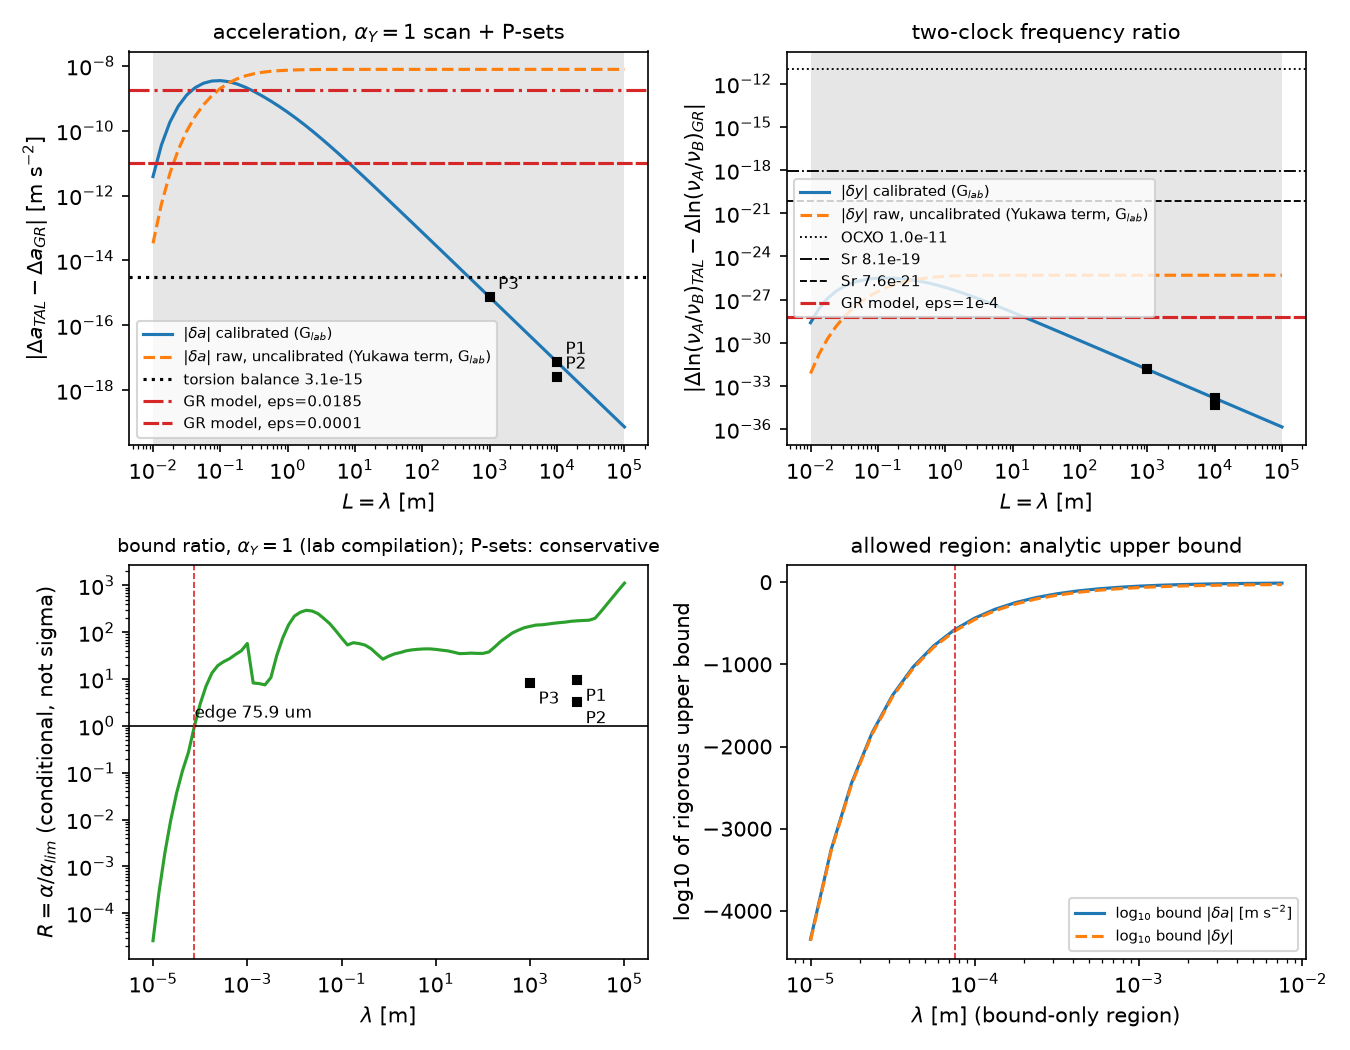
\includegraphics[width=0.9\textwidth]{../figures/fig_delta_vs_lambda.png}
\caption{Clock module figure: $|\delta a|$ and $|\delta y|$ against $L$ for $\alpha_Y=1$ and P1--P3; the ratio $R$; and, below
$10^{\V{quadLo}}\mU$, the analytic upper bound. The dashed raw curves are an uncalibrated illustration.}\label{fig:clock}
\end{figure}

\section{Yukawa bounds}\label{sec:bounds}
\subsection{BREN tower chain}\label{sec:bren}
The BREN module applies the continuation operator of the tower reports [Kasameyer 1989; Kammeraad 1990] to one source model and
compares the tower residual of a Yukawa term with the flat half-space form of V28 Step~27, at the model point
$\alpha=\V{brAlpha}$, $\lambda=\V{brLam}\kmu$. The source model uses synthetic ring radii ($\V{nRings}$ rings, $\V{nStations}$
stations; the reports give counts but not radii), a modern substitute DEM (Copernicus GLO-90, $\V{nGrid}\times\V{nGrid}$ cells
of $\V{cellM}\mU$) and uniform density. The original station and data chain is not reconstructed, so this is not an empirical
reanalysis of the experiment. The observable is referenced to $z_0=\V{zNull}\mU$ (K90); the V28 Step~27 numbers used
$z_0=0$ and are kept separate ($R=\V{RvNullTwo}$ at $\rho=\V{rho2000}\kgm$ and $\V{RvNullThree}$ at $\V{rho2670}\kgm$, reproduced exactly).
%CAV:bren_not_empirical
%CAV:z0_separate

Variants: A, spherical kernel with the raw truncated weights (sum $\V{wsum}$ with truncation at $\V{Rtrunc}\kmu$); B, weights
renormalised to zero sum; C, planar kernel; D, as A with a linear fit of the Newtonian bias. The truncation sensitivity of A
is an operator property, not a terrain signal, and the spread between A and B is not an uncertainty band. At the top point
($\V{zBN}\mU$, $\rho=\V{rho2200}\kgm$) the flat residual is $\V{topFlat}\uGal$; A gives $\V{topA}\uGal$, B gives
$\V{topB}\uGal$; the operator-only part of A is $\V{topOpA}\uGal$; the terrain part, common to all variants, is $\V{topTerr}\uGal$ ($\V{topTerrPct}\pct$ of the flat value).
As an independent check, the Newtonian terrain bias (direct minus continued) is $\V{nbias}\uGal$ against the report's
$\V{nbiasRep}\pm\V{nbiasRepSig}\uGal$, and $\V{nbiasKEN}\uGal$ at $\V{zKEN}\mU$ with $\rho=\V{rho1800}\kgm$ against about $\V{nbiasKENrep}\uGal$ in K89 (not tuned).
%CAV:A_truncation_not_terrain

Two conditional single-point comparisons are used. B89: the K89 residual $\V{kRes}\pm\V{kSig}\uGal$ at the
$\V{zKEN}\mU$ top, taken with the conservative sign and $k=\V{kSigma}$, gives an edge of $\V{edgeBEN}\uGal$. B90: the digitized
K90 Fig.~1 method-1 top point $+\V{yBN}\pm\V{sBN}\uGal$ at $\V{zBN}\mU$ (tower height $\V{hKN}\mU$) gives $\V{edgeBN}\uGal$.
Both use only the variance of one pre-selected point; the off-diagonal covariance with other heights does not enter a
single-point marginal test, which \file{check_single_point_marginal.py} confirms ($\V{nCovSame}$ of $\V{nCov}$ covariance
structures leave the edge unchanged). The K90 correlated $\chi^2$ analysis is not reproduced. Table~\ref{tab:brenR} gives the
ratios at $\lambda=\V{brLam}\kmu$ with density, height and construction per row.
%CAV:single_point_conditional
%CAV:K90_not_reproduced
\begin{table}[htbp]\centering\small\setlength{\tabcolsep}{5pt}
\caption{BREN: $R=\alpha/\alpha_{\rm lim}$ at $\lambda=\V{brLam}\kmu$, $z_0=\V{zNull}\mU$, $k=\V{kSigma}$. B89: K89 top point,
$\V{zKEN}\mU$; B90: K90 Fig.~1 top point, $\V{zBN}\mU$ (conditional single-point comparisons; not $\sigma$).}\label{tab:brenR}
\begin{tabular}{llccccc}\toprule
$\rho$ (\kgm) & bound & $R$ flat & $R$ A & $R$ B & $R$ C & $R$ D\\\midrule
\tabinput ../generated/tab_brenR.tex
\bottomrule\end{tabular}\end{table}

The DEM preparation uses a local equirectangular mapping; its east--west metric changes by up to $\V{metricPct}\pct$ at the
north and south edges. This is a declared limitation; it is not corrected, and it is not automatically a residual error of
that size.
%CAV:dem_metric

\begin{figure}[tbp]\centering
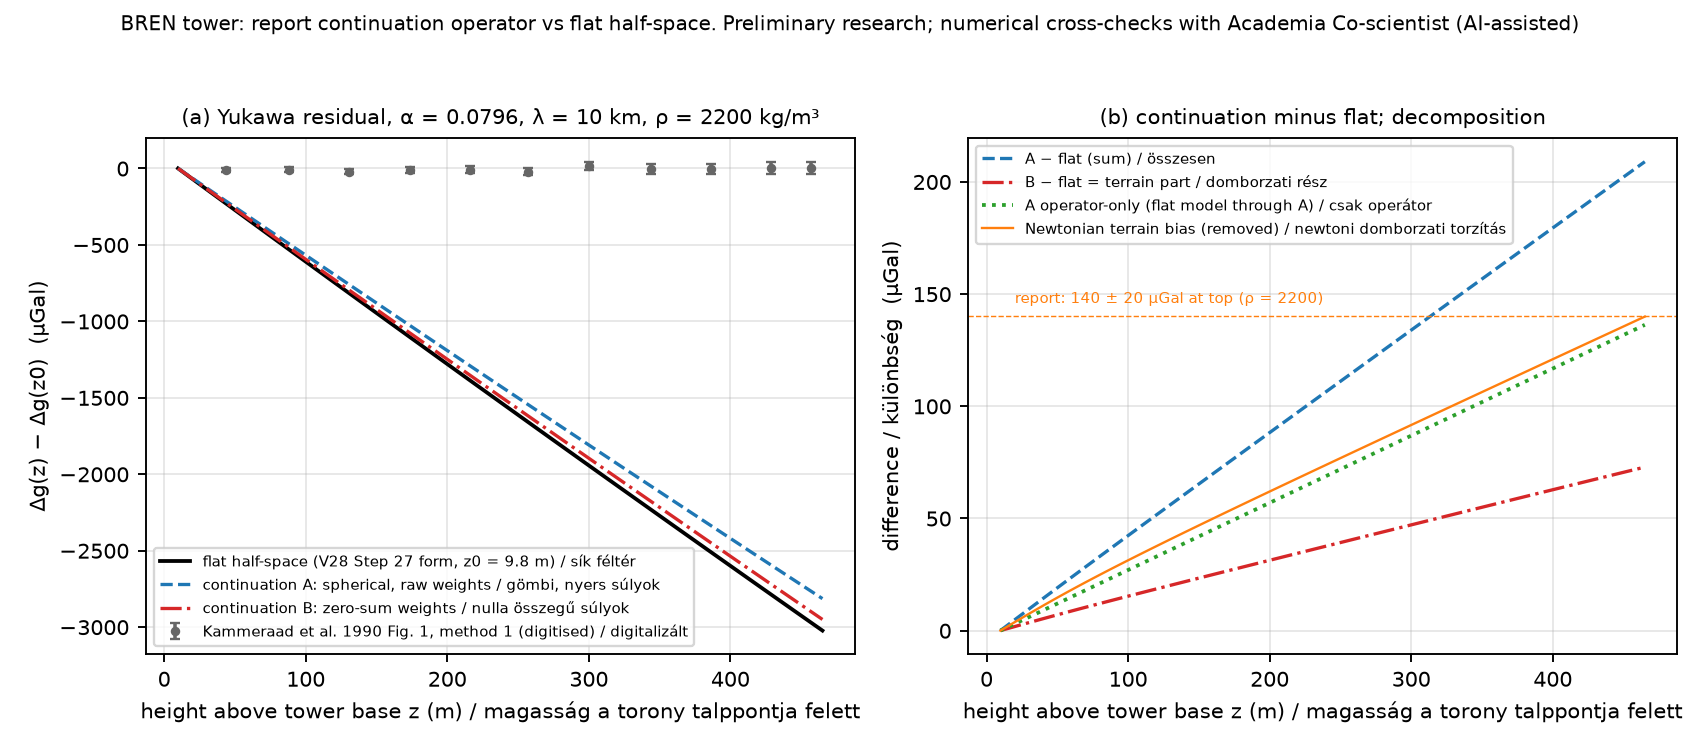
\includegraphics[width=\textwidth]{../figures/fig_residual_curve.png}
\caption{BREN module figure: (a) Yukawa residual against height for the flat half-space and variants A and B, with the
digitized K90 points; (b) continuation minus flat, decomposed.}\label{fig:bren}
\end{figure}

\subsection{Sub-centimetre chain}\label{sec:subcm}
The sub-cm module compares $\alpha=\V{scAlpha}$ with published short-range bounds ($\V{CL}\pct$ CL), vector-digitized from
Adelberger et al.\ 2003 and Lee et al.\ 2020, and with Table~11.4 of the Lee 2020 thesis ($\V{nThesis}$ rows).
The edges of the transition band are
$\V{eHust}\um$ (HUST 2020 $|\alpha|$ curve, reading interval $\V{loHust}$--$\V{hiHust}\um$),
$\V{eEW}\um$ (Eöt-Wash 2020 $|\alpha|$ curve, $\V{loEW}$--$\V{hiEW}\um$),
$\V{eAbs}\um$ (thesis $|\alpha_{95}|$, $\V{loAbs}$--$\V{hiAbs}\um$) and
$\V{ePlus}\um$ (thesis $+\alpha_{95}$, $\V{loPlus}$--$\V{hiPlus}\um$).
The band is not only a HUST sign question. From $\V{eHust}$ to about $\V{eEW}\um$, $\alpha$ is excluded only if the HUST 2020/2016
$|\alpha|$ curves are applied to $\alpha>0$. From about $\V{eEW}$ to $\V{ePlus}\um$ the two Eöt-Wash 2020 constructions differ
without any HUST curve: the thesis defines $\pm\alpha_{95}$ from the $\Delta\chi^2=\V{dchi}$ surface and $|\alpha_{95}|$ from a
normal integral; in the $\V{rowLam}\um$ row, $+\alpha_{95}=\V{rowPlus}>\alpha>|\alpha_{95}|=\V{rowAbs}$. The bounds are used as
published. The reading intervals come from the digitization and are not a physical uncertainty.
In the range $\lambda<\V{eHust}\um$ the value $\alpha=q$ is not excluded by the examined bounds; the search for newer bounds was
not exhaustive.
%CAV:band_not_hust_only
%CAV:digitization_not_physical
%CAV:not_exhaustive
\begin{table}[htbp]\centering\small
\caption{Sub-cm: $R=\alpha/\alpha_{\rm lim}$ at selected $\lambda$ (conditional, not $\sigma$).}\label{tab:subcmR}
\begin{tabular}{lcc}\toprule
$\lambda$ (\textmu m) & $R$, thesis $+\alpha_{95}$ & $R$, drawn $|\alpha|$ envelope\\\midrule
\tabinput ../generated/tab_subcmR.tex
\bottomrule\end{tabular}\end{table}

\begin{figure}[tbp]\centering
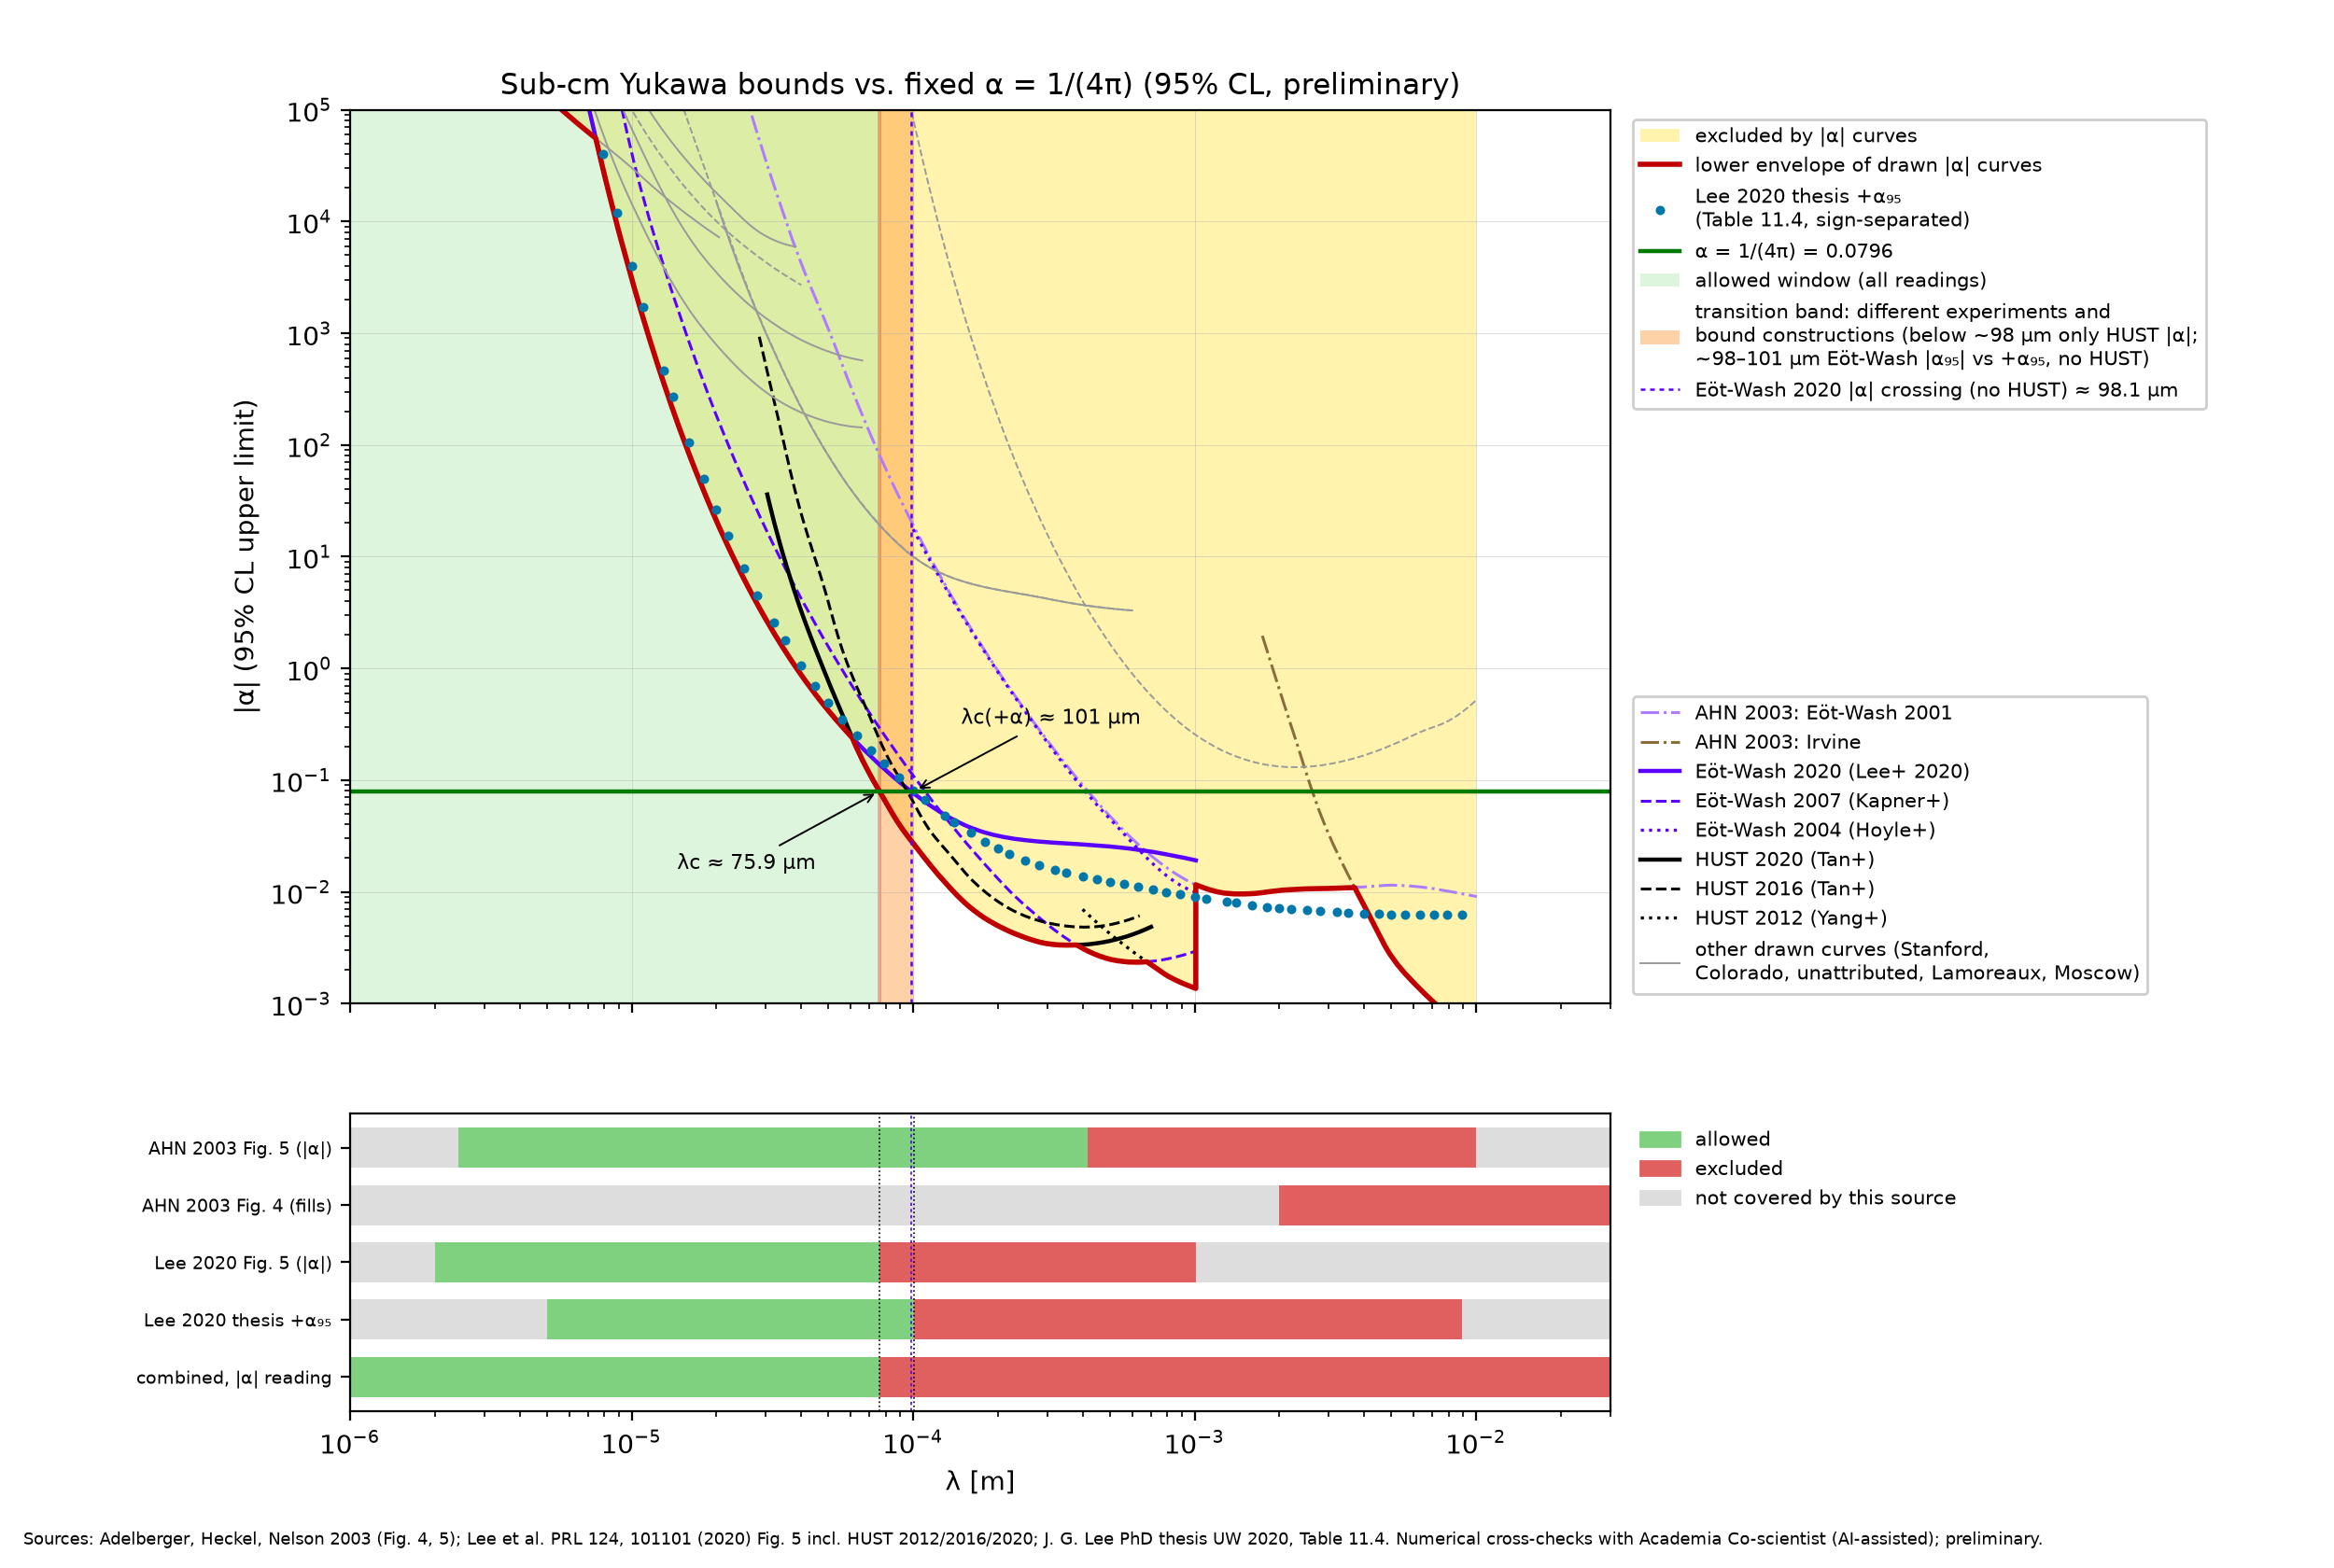
\includegraphics[width=\textwidth]{../figures/subcm_window_en.png}
\caption{Sub-cm module figure: drawn $|\alpha|$ bounds, the thesis $+\alpha_{95}$ points and $\alpha=1/(4\pi)$, with the
transition band.}\label{fig:subcm}
\end{figure}

\subsection{Ratios for P1--P3}\label{sec:ratio}
$R=\alpha/\alpha_{\rm lim}$ is a conditional ratio to a bound, not a significance: $R$ is not a number of standard deviations, and the bounds
are at different levels ($k=\V{kSigma}$ or $\V{CL}\pct$ CL for the laboratory and BREN single-point limits, $1\sigma$ for the
quoted K90 limit). Table~\ref{tab:bounds} combines the laboratory compilation (Adelberger et al.\ 2003 Fig.~4 above
$\V{eFigFour}\mmu$ with the sub-cm envelope) and the BREN B89 limits at $\rho=\V{rho2000}\kgm$ (variants A--C).
For P3 the K90 report limit $\V{aLimKN}$ at $\V{LP3}\kmu$ gives $R=\V{RKN}$; the project's B90 single-point value
$\V{aLimBNsp}$ ($R=\V{RBNsp}$) is a different construction, context only, and does not enter the conservative ratio.
Under U the redshift tests [Takamoto 2020; Grotti 2018] and the MICROSCOPE test [Touboul 2022] do not constrain the branch.
%CAV:R_not_sigma
\begin{table}[htbp]\centering\small\setlength{\tabcolsep}{3.5pt}
\caption{Bound ratios (conditional, not $\sigma$) and categories.}\label{tab:bounds}
\begin{tabular}{lcccccc}\toprule
set & $\alpha_{\rm lim}$ lab & $R$ lab & $\alpha_{\rm lim}$ BREN (A, B, C) & $R$ BREN & $R$ conservative & category\\\midrule
\tabinput ../generated/tab_bounds.tex
\bottomrule\end{tabular}\end{table}

\section{Conclusion}\label{sec:concl}
\begin{itemize}
\item The fixed branch (P1, P2, P3) is in category (b): $\delta y\ne0$ and $\delta a\ne0$, but the force is excluded by the
examined bounds, with smallest ratios $R=\V{RConsP1}$, $\V{RConsP2}$, $\V{RConsP3}$ (BREN, conditional on the examined models).
\item For $\alpha_Y=1$ the range $\lambda<\V{lamEdge}\um$ is not excluded by the examined bounds and is category (\V{catRem}):
there $\log_{10}|\delta a/(\mathrm{m\,s^{-2}})|\le\V{logDaEdge}$ and $\log_{10}|\delta y|\le\V{logDyEdge}$. In the widest
reading, up to $\V{ePlus}\um$, the bound gives $\log_{10}|\delta a/(\mathrm{m\,s^{-2}})|\le\V{logDaPlus}$ and
$\log_{10}|\delta y|\le\V{logDyPlus}$, category (\V{catBand}). This conclusion is for the declared geometry, whose closest
mass is $\V{dmin}\mU$ from the clocks.
\item No category (d) test exists for this branch in this setup. A short-range force test could probe $\alpha_Y=1$: at
$\lambda=\V{lamFifty}\um$ the drawn envelope gives $R=\V{Rfifty}$, so a torsion balance about $\V{ImpFifty}$ times more
sensitive there would reach $R=1$. This is a force experiment, not a clock experiment.
\end{itemize}
The checks reported here are technical (scripted reproduction, numeric comparison, negative controls); a passing check is not
an empirical confirmation of the branch. They were done as numerical cross-checks with Academia Co-scientist (AI-assisted).
%CAV:pass_technical

\appendix
\section{BREN operator}\label{app:bren}
The operator of K89 eq.~7 (= K90 eq.~2) is the spherical Poisson expansion to order $z/a$,
\begin{equation}
\Delta g(z)=\frac{z(1-2z/a)}{2\pi}\int\!\!\int\frac{\Delta g(0,r',\varphi)\,r'\,dr'\,d\varphi}{\big[r'^2+z^2(1-z/a)\big]^{3/2}},
\qquad a=\V{aEarth}\kmu,
\end{equation}
discretised into rings; ring $i$ (radii $r_1,r_2$) carries the mean of its sector stations times
$K_i(z)=z(1-2z/a)\big[(r_1^2+b^2)^{-1/2}-(r_2^2+b^2)^{-1/2}\big]$, $b^2=z^2(1-z/a)$, truncated at $\V{Rtrunc}\kmu$.
With $T$ the direct tower value and $P$ the continued value, $B_X(z)=[T_X(z)-T_X(z_0)]-[P_X(z)-P_X(z_0)]$ for Newton ($X=N$)
and Yukawa ($X=Y$), and the Yukawa residual is $\Delta g=G_\infty\alpha\rho\,(B_Y-B_N)$; in the flat limit it returns the
Step~27 form. Tower location $\V{towerLat}\degu$\,N, $\V{towerLon}\degu$\,W; $\V{nPrisms}$ signed terrain prisms.
Convergence at the top ($\rho=\V{rho2200}\kgm$, $\V{nConv}$ configurations besides the base): variant B changes by at most
$\V{convBmax}\uGal$; variant A runs from $\V{convAsixty}\uGal$ at $R_{\rm trunc}=\V{rtSixty}\kmu$ to $\V{convAfour}\uGal$ at
$\V{rtFour}\kmu$, as expected for the truncation term; the Newtonian bias spans $\V{convNmin}$--$\V{convNmax}\uGal$ and cancels in
the Yukawa residual. Table~\ref{tab:brenLam} shows $\alpha_{\rm lim}$ against $\lambda$ (B89, $\rho=\V{rho2000}\kgm$).
\begin{table}[htbp]\centering\small
\caption{BREN: $\alpha_{\rm lim}$ against $\lambda$ (B89, $\rho=\V{rho2000}\kgm$).}\label{tab:brenLam}
\begin{tabular}{lccc}\toprule
$\lambda$ (km) & flat & A & B\\\midrule
\tabinput ../generated/tab_brenLam.tex
\bottomrule\end{tabular}\end{table}

\section{Digitization and bound constructions}\label{app:digit}
The sub-cm curves were digitized from the vector content of the published figures (stroke paths, axis calibration by a fit
to all tick marks) and checked against a raster reading; the thesis table was parsed from the text layer. The digitized
values are frozen in the module, with SHA-256 sums, and are the input of its default run. The constructions differ: the drawn
$|\alpha|$ curves are bounds on $|\alpha|$; the thesis $\pm\alpha_{95}$ come from the $\Delta\chi^2=\V{dchi}$ surface;
$|\alpha_{95}|$ comes from the normal integral between $-|\alpha_{95}|$ and $+|\alpha_{95}|$. The older AHN 2003 Fig.~5 envelope
alone would put the edge at $\V{eAHN}\um$; the HUST 2016 curve crosses at $\V{eHustSix}\um$; the HUST-free gap is
$\V{eGap}\um$ wide. For BREN, B89 uses a value stated in K89 with $k=\V{kSigma}$, and B90 a point digitized from K90 Fig.~1; the
K90 limit itself ($1\sigma$, global multi-height correlated $\chi^2$) is quoted, not recomputed.
%CAV:constructions_differ

\section{Non-universal addon (outside the fixed branch)}\label{app:addon}
This appendix is an illustration outside the fixed branch and does not enter the decision. If the clock frequency had an
anomalous sensitivity, $\nu\propto e^{-(1+k_c)\phi}$, then $\delta y_{\rm extra}=-k_c\,\Delta(\phi_A-\phi_B)$, with $\phi$
normalized by $G_\infty$ (corrected in module version r4). Table~\ref{tab:addon} gives $\delta y_{\rm extra}$ for $k_c=1$ and
the $k_c$ needed for $S=\V{Sthr}$ at the Sr differential level. A long-range proxy with the Coulomb-energy fractions
$\xi_{\rm Ti}=\V{xiTi}$, $\xi_{\rm Pt}=\V{xiPt}$ and MICROSCOPE $|\eta|<\V{etaNF}$ gives $|k_c|\lesssim\V{kcMax}$; this proxy is
not transferred to $L=\V{LP3}$--$\V{LP1}\kmu$.
%CAV:addon_outside
\begin{table}[htbp]\centering\small
\caption{Non-universal addon (illustration only).}\label{tab:addon}
\begin{tabular}{lccc}\toprule
set & $G_\infty/G_{\rm lab}$ & $\delta y_{\rm extra}$ ($k_c=1$) & $k_c$ for $S=\V{Sthr}$\\\midrule
\tabinput ../generated/tab_addon.tex
\bottomrule\end{tabular}\end{table}

\section*{Data and code availability}\label{sec:avail}
The three module archives are in the publication set, unchanged, with SHA-256 sums:
\begin{itemize}\setlength{\itemsep}{0pt}
\item \file{tal_branch_clock_accel_test_r4.zip} (clock and acceleration, main analysis);
\item \file{bren_continuation_zenodo_r4.zip} (BREN tower continuation);
\item \file{subcm_yukawa_window_zenodo_r4.zip} (sub-centimetre Yukawa window).
\end{itemize} The article sources, the claim--source
table and its check script are in \file{article/}. Concept DOI of the TAL work: \doi{10.5281/zenodo.22983681}; related records:
V20 \doi{10.5281/zenodo.23540741}, V26 \doi{10.5281/zenodo.23727585}, V28 \doi{10.5281/zenodo.23814053}.
Licence: CC BY-NC 4.0 International; third-party documents and data remain under their own terms.

\section*{References}
\footnotesize
\begin{itemize}\setlength{\itemsep}{0pt}
\item E. G. Adelberger, B. R. Heckel, A. E. Nelson, Annu.\ Rev.\ Nucl.\ Part.\ Sci.\ 53, 77 (2003), arXiv:hep-ph/0307284.
\item J. G. Lee, E. G. Adelberger, T. S. Cook, S. M. Fleischer, B. R. Heckel, Phys.\ Rev.\ Lett.\ 124, 101101 (2020), arXiv:2002.11761.
\item J. G. Lee, PhD thesis, University of Washington (2020), \url{https://hdl.handle.net/1773/45542}, Table 11.4.
\item W.-H. Tan et al., Phys.\ Rev.\ Lett.\ 124, 051301 (2020); W.-H. Tan et al., Phys.\ Rev.\ Lett.\ 116, 131101 (2016).
\item D. J. Kapner et al., Phys.\ Rev.\ Lett.\ 98, 021101 (2007); C. D. Hoyle et al., Phys.\ Rev.\ D 70, 042004 (2004).
\item P. Kasameyer et al., UCRL-101001 (1989), OSTI 6190822 [K89]; J. Kammeraad et al., UCRL-JC-103562 (1990), OSTI 6993119 [K90].
\item T. Bothwell et al., Nature 602, 420 (2022); M. Aeppli et al., Phys.\ Rev.\ Lett.\ 133, 023401 (2024).
\item S. Schlamminger et al., Phys.\ Rev.\ Lett.\ 100, 041101 (2008); P. Touboul et al., Phys.\ Rev.\ Lett.\ 129, 121102 (2022).
\item M. Takamoto et al., Nat.\ Photon.\ 14, 411 (2020); J. Grotti et al., Nat.\ Phys.\ 14, 437 (2018).
\item Oscilloquartz 8662/8663 specification (March 2003); CODATA 2018 recommended values; Copernicus GLO-90 DEM.
\end{itemize}
\end{document}
